\documentclass[a4paper,12pt]{report}
\addtolength{\oddsidemargin}{-1.cm}
\addtolength{\textwidth}{2cm}
\addtolength{\topmargin}{-2cm}
\addtolength{\textheight}{3.5cm}
\newcommand{\HRule}{\rule{\linewidth}{0.5mm}}
\setcounter{secnumdepth}{5}
\setcounter{tocdepth}{3}
\makeindex

\usepackage{longtable}
\usepackage{graphicx}
\usepackage{makeidx}
\usepackage{hyperref}
\usepackage{verbatim}
\usepackage{placeins}

\hypersetup{
    colorlinks=true,
    linkcolor=blue,
    filecolor=magenta,      
    urlcolor=cyan,
}


% define the title
\author{Ambitious Design}
\title{ Software Requirements Specifications and Technology Neutral Process Design}
\begin{document}
\setlength{\parskip}{6pt}

% generates the title
\begin{titlepage}

\begin{center}
% Upper part of the page           
\textsc{\LARGE Willburg Outdoor PTY(ltd.)}\\[1.5cm]
\textsc{\Large Smart Image Identifier }\\[1.0cm]
\textsc{\Large Version 1.0 }\\[0.5cm]
% Title
\HRule \\[0.4cm]
{ \huge \bfseries  Application Requirements Specifications and Design}\\[0.4cm]
\HRule \\[0.4cm]
% Author and supervisor
\begin{minipage}{0.4\textwidth}
\begin{flushleft} \large
\emph{Author:}\\
Stephen {Swanepoel}
\end{flushleft}
\end{minipage}
\begin{minipage}{0.4\textwidth}
\begin{flushright} \large
\emph{} \\
u11032091
\end{flushright}
\end{minipage}
\begin{minipage}{0.4\textwidth}
\begin{flushleft} \large
Dian {Veldsman}
\end{flushleft}
\end{minipage}
\begin{minipage}{0.4\textwidth}
\begin{flushright} \large
\emph{} \\
u12081095
\end{flushright}
\end{minipage}
\begin{minipage}{0.4\textwidth}
\begin{flushleft} \large
Killian {Kieck}
\end{flushleft}
\end{minipage}
\begin{minipage}{0.4\textwidth}
\begin{flushright} \large
\emph{} \\
u12252213
\end{flushright}
\end{minipage}


{\large \today}
\end{center}
\end{titlepage}
\footnotesize
\normalsize

\renewcommand{\thesection}{\arabic{section}}
\newpage

\section {Background}
Rhino poaching is currently at a crisis point. By the end of 2015, the number of African rhinos killed by poachers had increased for the sixth year in a row with at least 1,338 rhinos killed by poachers across Africa in 2015. South Africa has by far the largest population of rhinos in the world and is an incredibly important country for rhino conservation. However rhino poaching levels have dramatically escalated over recent years. \\
\\The South African farm attacks are an ongoing trend of violent attacks on farmers in South Africa. Between 1994 and March 2012, there have been 361,015 murders in South Africa. While the police are supposed to regularly visit commercial farms to ensure security, they claim they cannot provide effective protection due to the wide areas that need to be covered and a lack of funding.\\
\\Willburg Outdoor is company that is passionate about the South Africa. With this passion comes the need to protect its farmers and it animals from those who intend to harm them.The client intends to use the system to fight these two problems by alerting the user of the Willburg camera of the identification in an effort to potentially stop a crime or poaching from accuring. This will hopefully deter future poachers and farm attackers.

\subsection {Smart Image Identification System}
The Smart Image Identifier will consist of 3 modules:
	\begin {itemize}
		\item Process Image
		\item Identification
		\item ImageSorting
	\end {itemize}

The above mentioned module will consist of the following:
	\subsubsection {Process Image}
		This module consists of 
			\begin {itemize}
				\item Processing an image inorder to prepare it for human identification
			\end {itemize}

	\subsubsection {Identification}
		This module consists of
			\begin {itemize}
				\item Identifiying if there is a human in the image
			\end {itemize}

	\subsubsection {ImageSorting}
		This module consists of
			\begin {itemize}
				\item Sorting image into baskets and groupings
			\end {itemize}


\section {Vision and Objectives}
	\subsection {Vision}
	 The client for this project, Willburg Outdoor PTY(ltd.), has called for the design of an application that will assess an images, 	identify a human(s) in the image. If a human has been identified by the system, a call must then be set out to warn a user. The main idea behind the project is to be able to alert the user, of the Willburg camera, that a human has been identified so that the user will be informed about the movement around the camera.

	\subsection {Objectives}
	The main objectives of the Smart Image Identifier system is to
	\begin {itemize}
		\item Assesses the image by sorting the image into baskets and groupings inorder to improve the clients database on a constant basis.
		\item Identify if a human is present in the picture.
	\end {itemize}


\section {Process Image}
The ImageProcessing module provides the functionality of manipulating and processing an image inorder for the system to better detect  humans.
	\FloatBarrier
	\subsection {Scope}
		The scope of the ImageProcessing module include:
			\begin {itemize}
				\item Submit image to be processed
				\item Process image
			\end {itemize}

	\FloatBarrier
	\subsection {Domain Model}
		The image processor uses an image inorder to create an instance of the processed image
		\begin{figure}[htb]
			\centering
			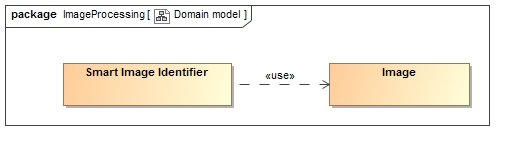
\includegraphics [scale=0.5]{../Diagrams/ProcessImage_Domain_model.jpg}
			\caption{Domain model for the Process Image model}
		\end{figure}	

		\FloatBarrier
		\subsubsection {Service contract}
			\begin{figure}[htb]
				\centering
				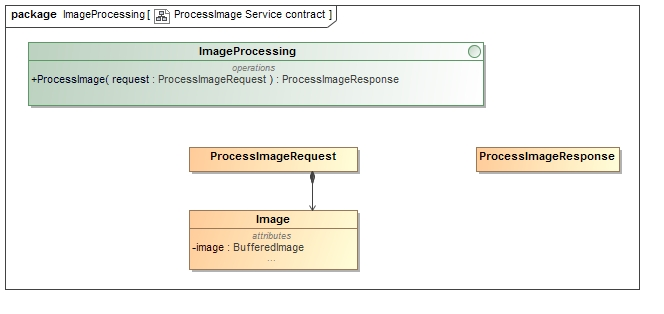
\includegraphics [scale=0.5]{../Diagrams/ProcessImage_Service_contract.jpg}
				\caption{ImageProcessing service contract}
			\end{figure}	
			To process an image the following must hold:
			\begin {itemize}
				\item 
			\end {itemize}

			If an error occurs during reading the image an IOException is thrown.In addition, the service will be refused if the request does not comply to the data structure specification.
		
		\FloatBarrier
		\paragraph {Functional requirements}

		\FloatBarrier
		\paragraph {processDesign}
		An image is first processed into a buffered image. The buffered image's data is then stored within a Mat object which is then used to manipulate, such as enlarging, greyscaling and equalization inorder to better improve the detection of a person. The processed image is then sent as request to identify a human.
		\begin{figure}[htb]
			\centering
			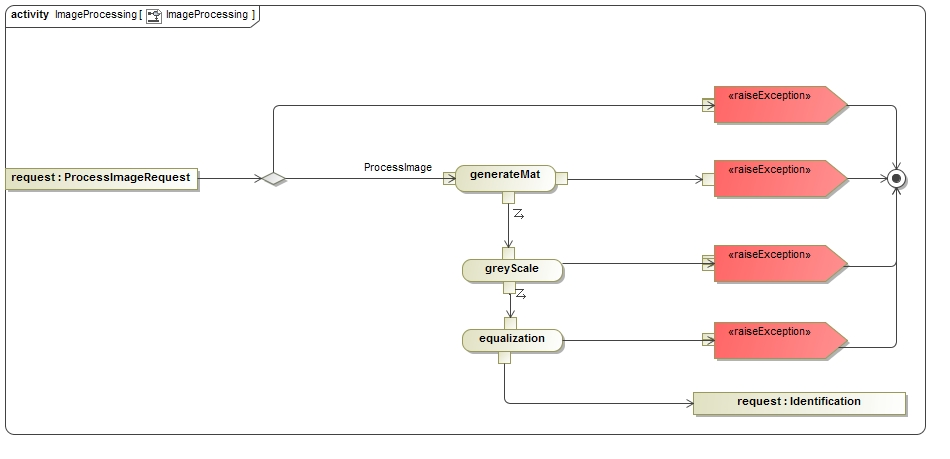
\includegraphics [scale=0.5]{../Diagrams/ImageProcessing.jpg}
			\caption{Process image process design}
		\end{figure}	

\FloatBarrier	
\section {Identification}
The Identification module provides the functionality of identification of humans with OpenCV

	\FloatBarrier	
	\subsection {Scope}
	The scope of the Identification module include:
		\begin {itemize}
			\item Submit processed image to do identification on
			\item Identify humans
		\end {itemize}

	\FloatBarrier	
	\subsection {Domain Model}
		The processed image is sent to the identification module where the OpenCV's built in algorithm is used(HOG) and set to the default "people detector".
		\begin{figure}[htb]
			\centering
			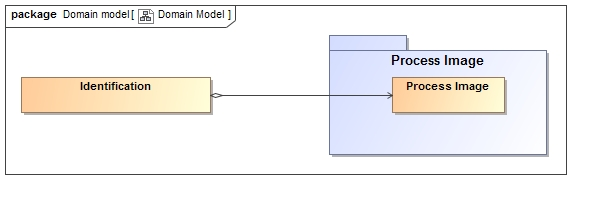
\includegraphics [scale=0.5]{../Diagrams/Identification_Domain_Model.jpg}
			\caption{Identification Domain model}
		\end{figure}	

		\FloatBarrier	
		\subsubsection {Service contract}
			\begin{figure}[htb]
				\centering
				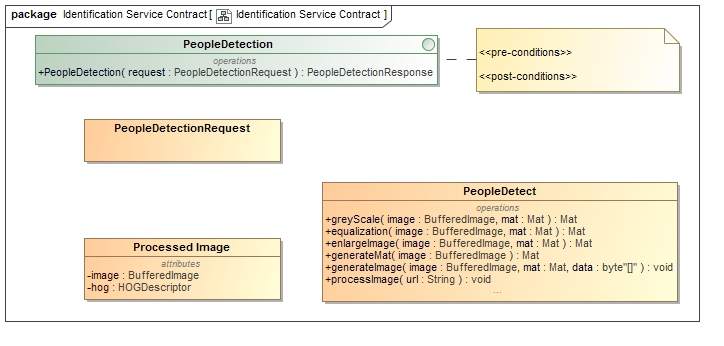
\includegraphics [scale=0.5]{../Diagrams/Identification_Service_Contract.jpg}
				\caption{Identification process design}
			\end{figure}	

			\FloatBarrier				
			\paragraph {Functional requirements}
			
			\FloatBarrier	
			\paragraph {processDesign}
				\begin{figure}[htb]
					\centering
					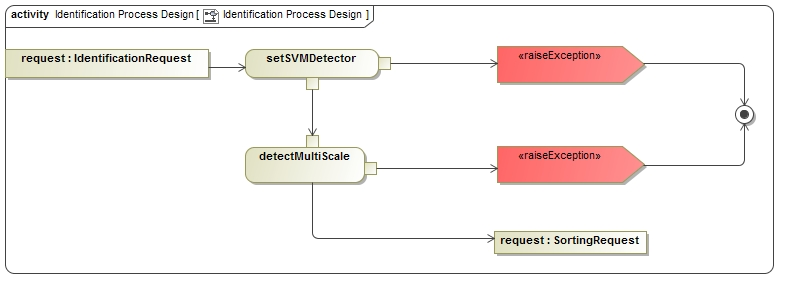
\includegraphics [scale=0.5]{../Diagrams/Identification_Process_Design.jpg}
					\caption{Identification process design}
				\end{figure}	

\section {ImageSorting}
		\FloatBarrier	
		\subsection {Scope}
		The scope of the ImageSorting module include:
			\begin {itemize}
				\item Submit image to be processed
				\item Process image
			\end {itemize}
	
	\FloatBarrier		
	\subsection {Domain Model}
		\FloatBarrier	
		\subsubsection {Service contract}		
		\begin{figure}[htb]
			\centering
			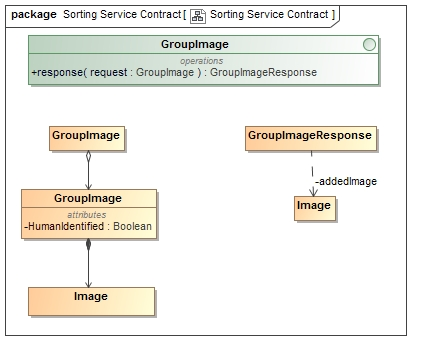
\includegraphics [scale=0.5]{../Diagrams/Sorting_Service_Contract.jpg}
			\caption{Identification process design}
		\end{figure}
		
			\FloatBarrier	
			\paragraph {Functional requirements}

			\FloatBarrier	
			\paragraph {processDesign}
			\begin{figure}[htb]
				\centering
				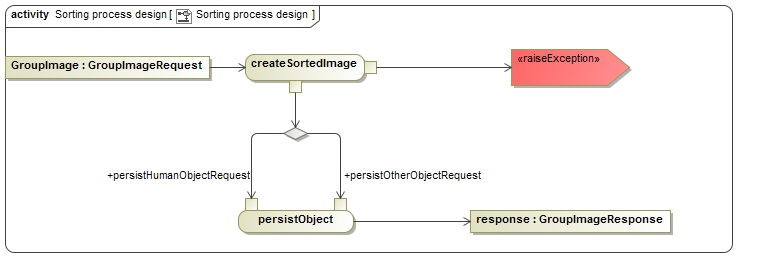
\includegraphics [scale=0.5]{../Diagrams/Sorting_process_design.jpg}
				\caption{Identification process design}
			\end{figure}	



\end{document}